\documentclass[a4paper,10pt]{article}
\usepackage[utf8]{inputenc}
\usepackage{amsmath, amsfonts, graphicx}
%opening
\title{}
\author{}

\begin{document}

\maketitle

\begin{abstract}

\end{abstract}

\section{Fundamental matrix}

Let us have 2 shots of the same scene made with slightly rotated cameras so that the transformation between the camera coordinate system $K'$ and $K$ is given via the rotation matrix $R$ and the translation vector $T$, i.e. the coordinates $X$ and $X'$ of the point $M$ are related as follows:

\begin{equation}
 X = RX'+T
\end{equation}
The inverse transformation reads

\begin{equation}
 X'=R^TX-R^TT
\end{equation}


A point $M$ is projected on images on points $\xi$ and $\xi'$ respectively as shown in Fig. \ref{fig:epipoles}.

The line joining the camera centers $C$ and $C'$ intersects with the image plains in the points $e$ and $e'$ - the {\it epipoles}.

\begin{figure}[h]
\centering
 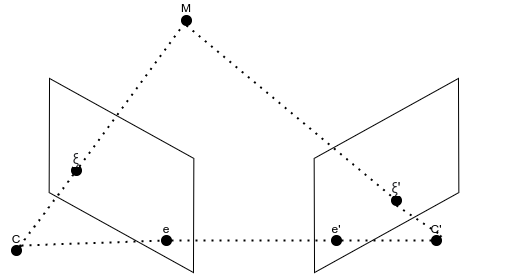
\includegraphics[width=0.9\textwidth]{../../images/epipoles.png}
 \caption{Epipolar geometry }
 \label{fig:epipoles}
\end{figure}

{\bf Proposition:} For any non-identical euclidean transformation $(R, T)$ there exists a matrix $F\equiv F(R, T)$ such that 

\begin{equation}
 X^T F X' = 0. 
\end{equation}

{\bf Proof:} It is easy to derive the coordinates of the epipoles in both coordinate systems. Since the coordinate of each camera center in its own coordinate system is $(0,0,0)$, the homogeneous coordinates of $e$ and $e'$ simply read:
\begin{equation}
 e = T, \quad e'= - R^TT
\end{equation}

Each point $\xi$ on the left image corresponds to a ray $\lambda \xi$ in the 3D-space. It is obvious from the construction that this ray corresponds to a line joining $\xi'$ and $e'$ on the second image. On the other hand, a line passing through 2 homogeneous points $x$ and $y$ is given by a cross product

\begin{equation}
 l = x \times y. 
\end{equation}

This automatically satisfies the condition 
$$
l\cdot x = l\cdot y = 0.
$$

Applying this to the points $e'$ and $X'$ gives us

\begin{equation}
 l' = e'\times X' = -(R^TT)\times (R^T X - R^T T) = -(R^TT)\times(R^TX)\equiv F X
\end{equation}
By construction $X'\cdot l' = 0$, and this proves the statement.

\end{document}
